\chapter{Evaluation}

Explaining how your software was tested (using different datasets or in different environments), statistical evaluation of performance, results of user evaluation questionnaires, etc.

\section{Examples of a figure}

Example of a mathematical formula:
\begin{equation}
  ADD = \sum_{i=1}^{M}|<D(n+1,i)>-<D(n,i)>|
  \label{add}
\end{equation}

Example of a figure. that is allowd to float in the whole chapter!

\begin{figure}[ht!]
\begin{center}
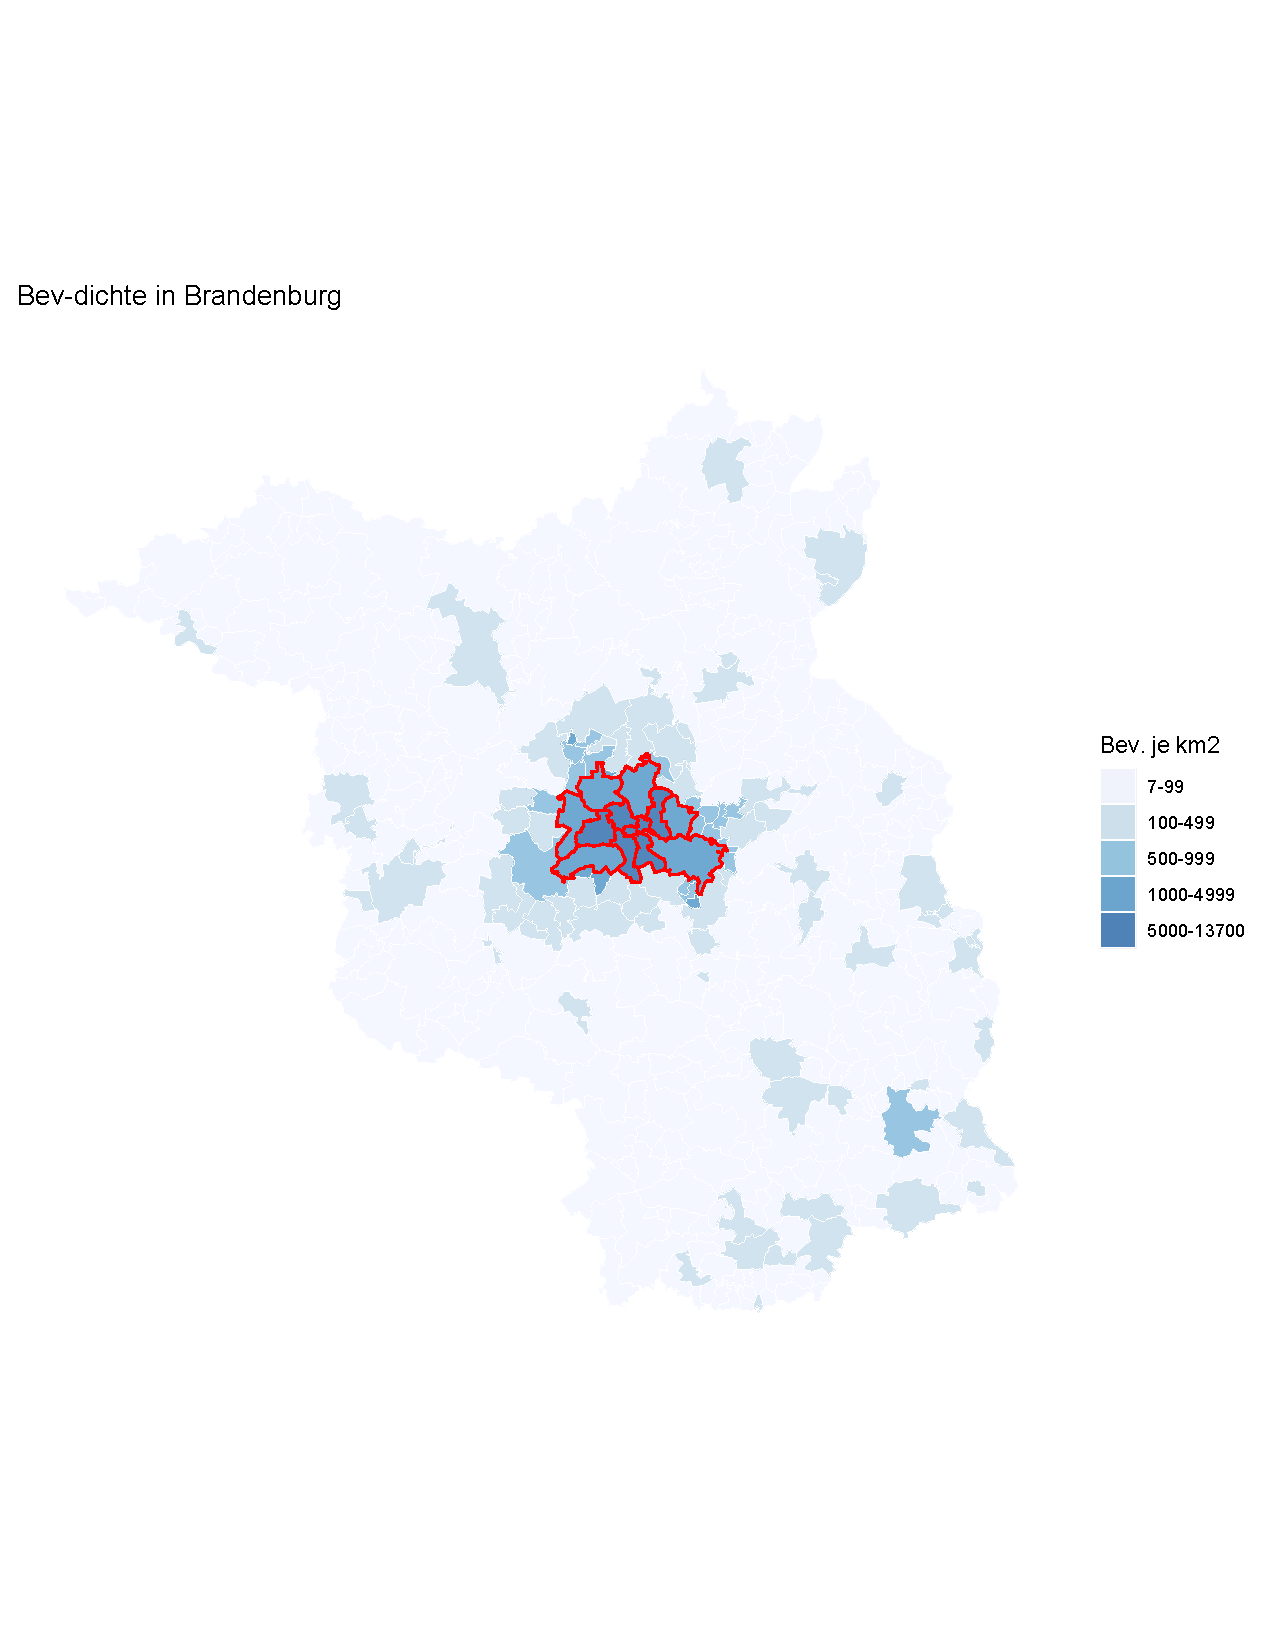
\includegraphics[scale=0.5]{body/figures/Gem-2.pdf}
\end{center}
\caption[Bevölkerungsdichte in Berlin und Brandenburg]{Bevölkerungsdichte in Berlin und Brandenburg im Jahre 2013. Weitere Details hier eingeben. Grafik erstellt mit Daten aus: Quelle}
%Source:
\label{fig_bb1}
\end{figure}

%After more text, here is an example of reference to a figure in the text (Fig.~\ref{fig_bb1}).

\section{Examples of a table}
\begin{table}
    \begin{center}
    \begin{tabular}{|l|c|c|r|}
    \hline
    {\sc Organism}  &  {\sc Accession no.}  & {\sc Genome size} (bp)  & {\sc No. CDS} \\
    \hline
    {\it Mesorhizobium loti}          & NC\_002678 & 7036071 & 6743 \\
    %\hline
    {\it Sinorhizobium meliloti}      & NC\_003047 & 3654135 & 3359 \\
    %\hline
    {\it Bradyrhizobium japonicum}    & NC\_004463 & 9105828 & 8317 \\
    %\hline
    {\it Rhodopseudomonas palustris}  & NC\_005296 & 5459213 & 4813 \\
    %\hline
    {\it Bartonella quintana}         & NC\_005955 & 1581384 & 1142 \\
    %\hline
    {\it Bartonella henselae}         & NC\_005956 & 1931047 & 1488 \\
    %\hline
    {\it Rickettsia typhi}            & NC\_006142 & 1111496 & 837 \\
    %\hline
    {\it Beijerinckia indica}         & NC\_010581 & 4170153 & 3569 \\
    \hline
    \end{tabular}
    \end{center}
    \caption{Whole-genome sequences used in this study}
    \label{table_genomes}
    \end{table}
    
